\documentclass{article}

\usepackage[hidelinks]{hyperref}
\usepackage{enumitem}
\usepackage{todonotes}
\usepackage{listings}
\usepackage{color}
\usepackage[plain]{fancyref}
\usepackage{subfigure}
\usepackage{wrapfig}
\usepackage{float}
\usepackage{graphicx}
%\usepackage{marginnote}
%REMOVE BELOW COMMAND TO GET NORMAL VIEW
%\usepackage[top=1.5cm, bottom=1.5cm, outer=5cm, inner=2cm, heightrounded, marginparwidth=2.5cm, marginparsep=2cm]{geometry}

\definecolor{light-gray}{gray}{0.95}
\lstset{mathescape,
		basicstyle=\ttfamily,
		backgroundcolor=\color{light-gray}
		}
\lstset{numbers=right, 
                numberstyle=\tiny,
                escapechar=\&,
                breaklines=true,
                backgroundcolor=\color{light-gray},
                %xleftmargin=\parindent,
                %xleftmargin=1cm,
                %xrightmargin=\parindent,
                numbersep=5pt}

%\newcommand*{\UTlogo}{\fbox{$\mathcal{UT}$}}
\newcommand*{\UTlogo}{
\includegraphics{Figures/utlogo.png}}

%---------------------------------------------------------------------------
%	TITLE PAGE
%	Page taken from: http://www.latextemplates.com/template/vertical-line-title-page
%---------------------------------------------------------------------------
\newcommand*{\titleGM}{\begingroup
\hbox{
\hspace*{0.2\textwidth}
\rule{1pt}{\textheight}
\hspace*{0.05\textwidth}
\parbox[b]{0.75\textwidth}{

%{\noindent\LARGE \textit{Note: Margin notes version!} \\ \textit{Note: Spell check should be done!} } \\[2\baselineskip]
{\noindent\Huge\bfseries Stairwalker \\[0.5\baselineskip] User Manual}\\[1\baselineskip]
%{\large \textit{We could write something here}}\\[4\baselineskip]
{\large Document authors: \\[0.2\baselineskip]
 \Large \textsc{- Dennis Muller (UT)} \\[0.25\baselineskip]
 \Large \textsc{- Jochem Elsinga (UT)} \\[0.25\baselineskip]
 \Large \textsc{- Maurice van Keulen (UT)} \\[0.4\baselineskip]
 \large Software developers: \\[0.2\baselineskip]
 \Large \textsc{- Andreas Wombacher (UT)} \\[0.25\baselineskip]
 \Large \textsc{- Jan Flokstra (UT)} \\[0.25\baselineskip]
 \Large \textsc{- Henke Pons (Arcadis)} \\[0.25\baselineskip]
 \Large \textsc{- Niek de Vries (Arcadis)} \\[0.25\baselineskip]
}

\vspace{0.05\textheight}
{\noindent\fbox{
\includegraphics{COMMIT_logo_RGB.pdf}}}

\vspace{0.05\textheight}
\begin{tabular}{ll}
\begin{minipage}[h]{1.2in}

\includegraphics[width=3cm]{ctit.jpg}
\vspace{-0.5cm}
\end{minipage}
&
\begin{minipage}[t]{3in}
\vspace{-3.6ex}
\textbf{CTIT Technical Report CTIT-TR-15-09}\\
Centre for Telematics and Information Technology\\
P.O.\ Box 217, 7500 AE\\
Enschede, The Netherlands
\end{minipage}\\
\end{tabular}

\vspace{0.06\textheight}
{21 December 2015}\\[0.5\baselineskip]
{\noindent \UTlogo}\\[\baselineskip]
}}
\endgroup}

%---------------------------------------------------------------------------
%	DOCUMENT
%---------------------------------------------------------------------------
\begin{document}

\pagestyle{empty}

\titleGM

\tableofcontents
\pagebreak
\pagestyle{plain}
%---------------------------------------------------------------------------
%	Sections
%---------------------------------------------------------------------------

\section{Introduction}
Geographical data are typically visualized using various information layers
that are displayed over a map. Interactive exploration by zooming and
panning actions needs real-time re-calculation. A common operation in
calculating with multidimensional data is the computation of aggregates.
For layers containing aggregated information derived from voluminous data
sets (see for example Figure~\ref{fig:NL-screenshot}), such real-time
exploration is impossible using standard database technology. Calculations
require too much time.

The University of Twente has developed \emph{``Stairwalker''}: database
technology that accurately aggregates data so that they can geographically
be explored in real-time. The technology is a plug-in to common open
source technology.

Its core is the \emph{pre-aggregate index}: a database index that cleverly
pre-calculates aggregation values such that it can obtain exact aggregation
results from voluminous data with high performance.  A fast calculation
allows to fully recalculate the result for even the slightest movement of
the map, such as a panning or zooming action, without loss of accuracy.
Thanks to this indexing mechanism, we can provide a scalable real-time
calculation: an order of magnitude larger dataset requires only one
additional aggregation level.

In geo data visualization, the ability to quickly develop new information
layers is important. Although many solutions exist, there is a niche: the
combination of visualizing aggregation information, interactive data
exploration in real-time, Big Data, calculating exact numbers instead of
approximations, and doing so with common open source technology. Our
technology for the first time integrates all these features.

\begin{figure}[t]
\centering
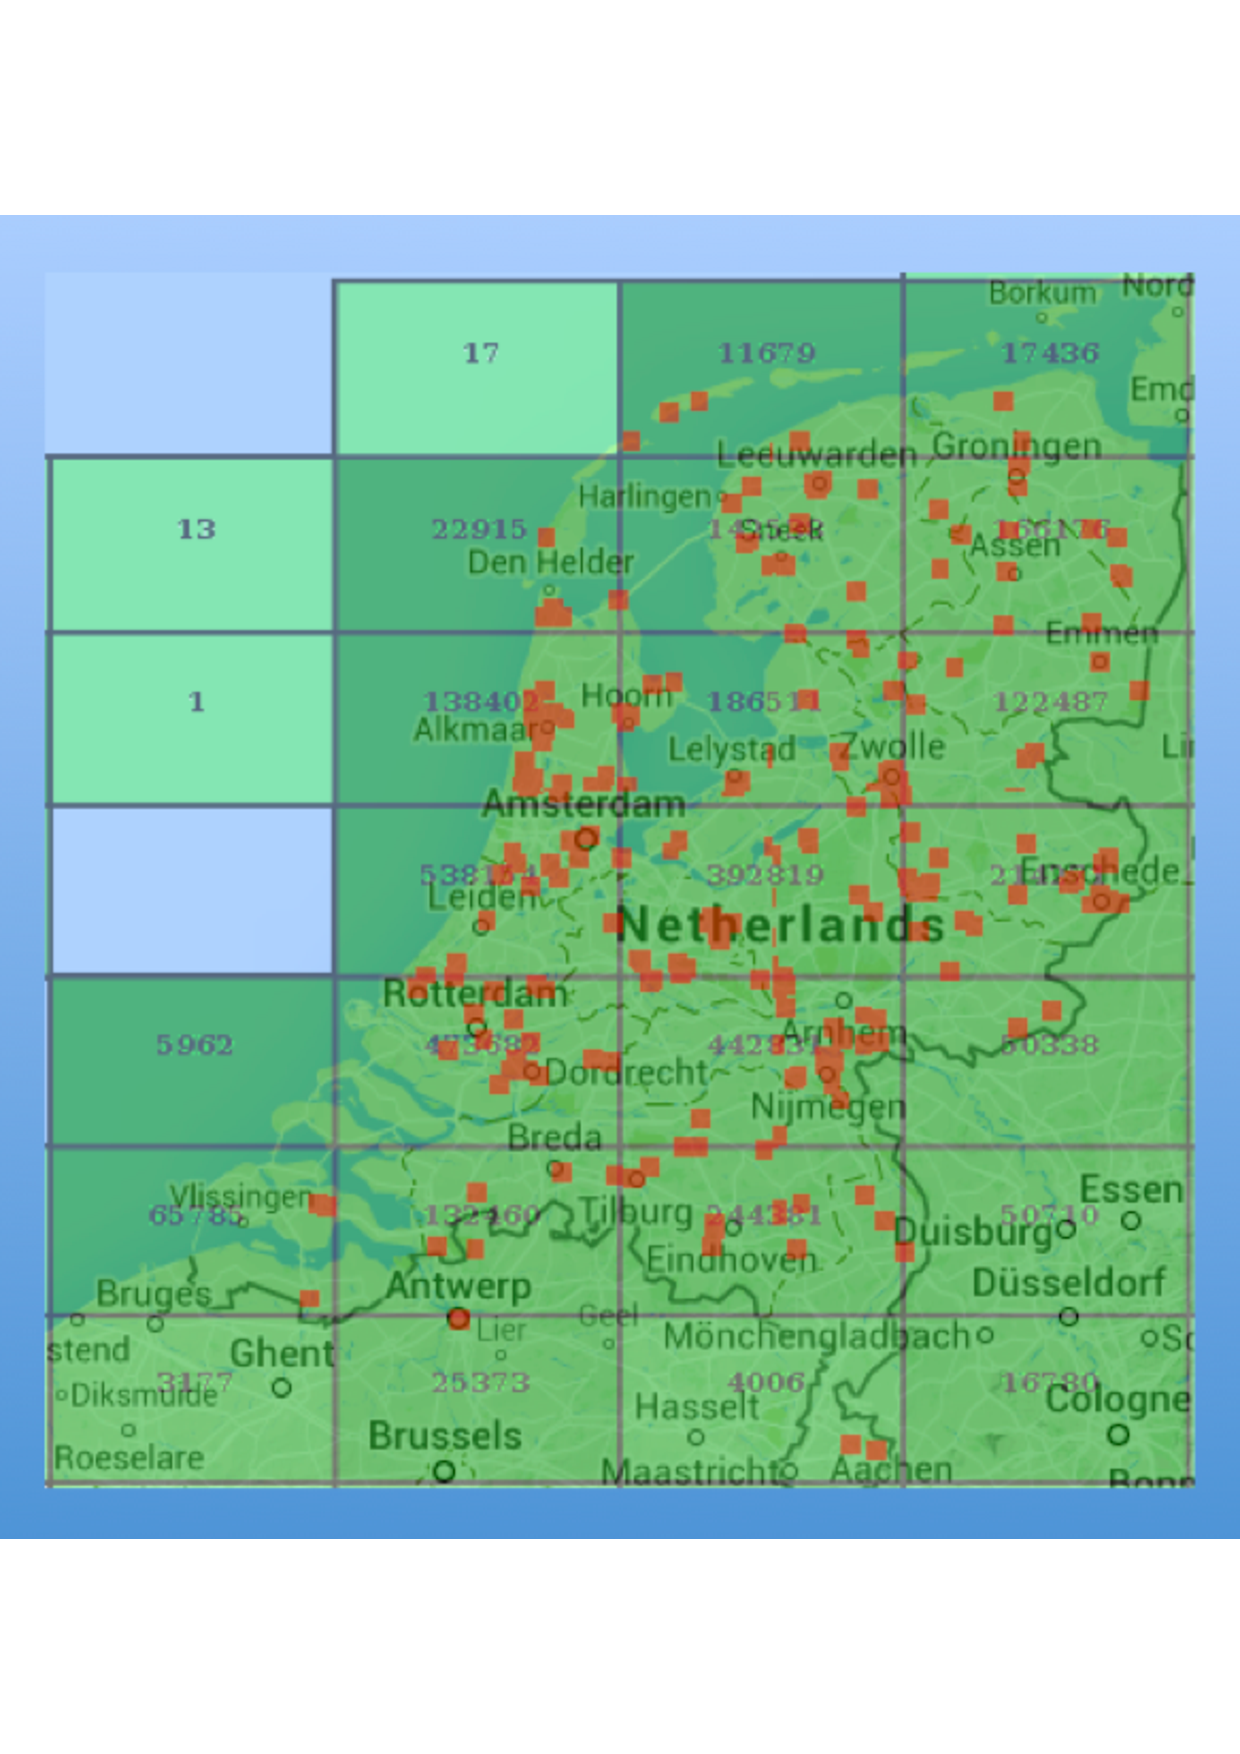
\includegraphics[height=4in]{Figures/NL-screenshot.pdf}
\caption{Twitter hotspot detection in The Netherlands, using a coarse grid.
The numbers inside the grid cells on the map require an aggregation
operation in the database.}
\label{fig:NL-screenshot}
\end{figure}


Our research partners are the companies Arcadis and Nspyre. They both have
struggled with this combination of requirements in many of their projects.
Our database index technology is not specific to geographical data. It can
be used with all types of multidimensional data. Visualization in business
intelligence or eScience can also benefit from it.

\begin{figure}[t]
\centering
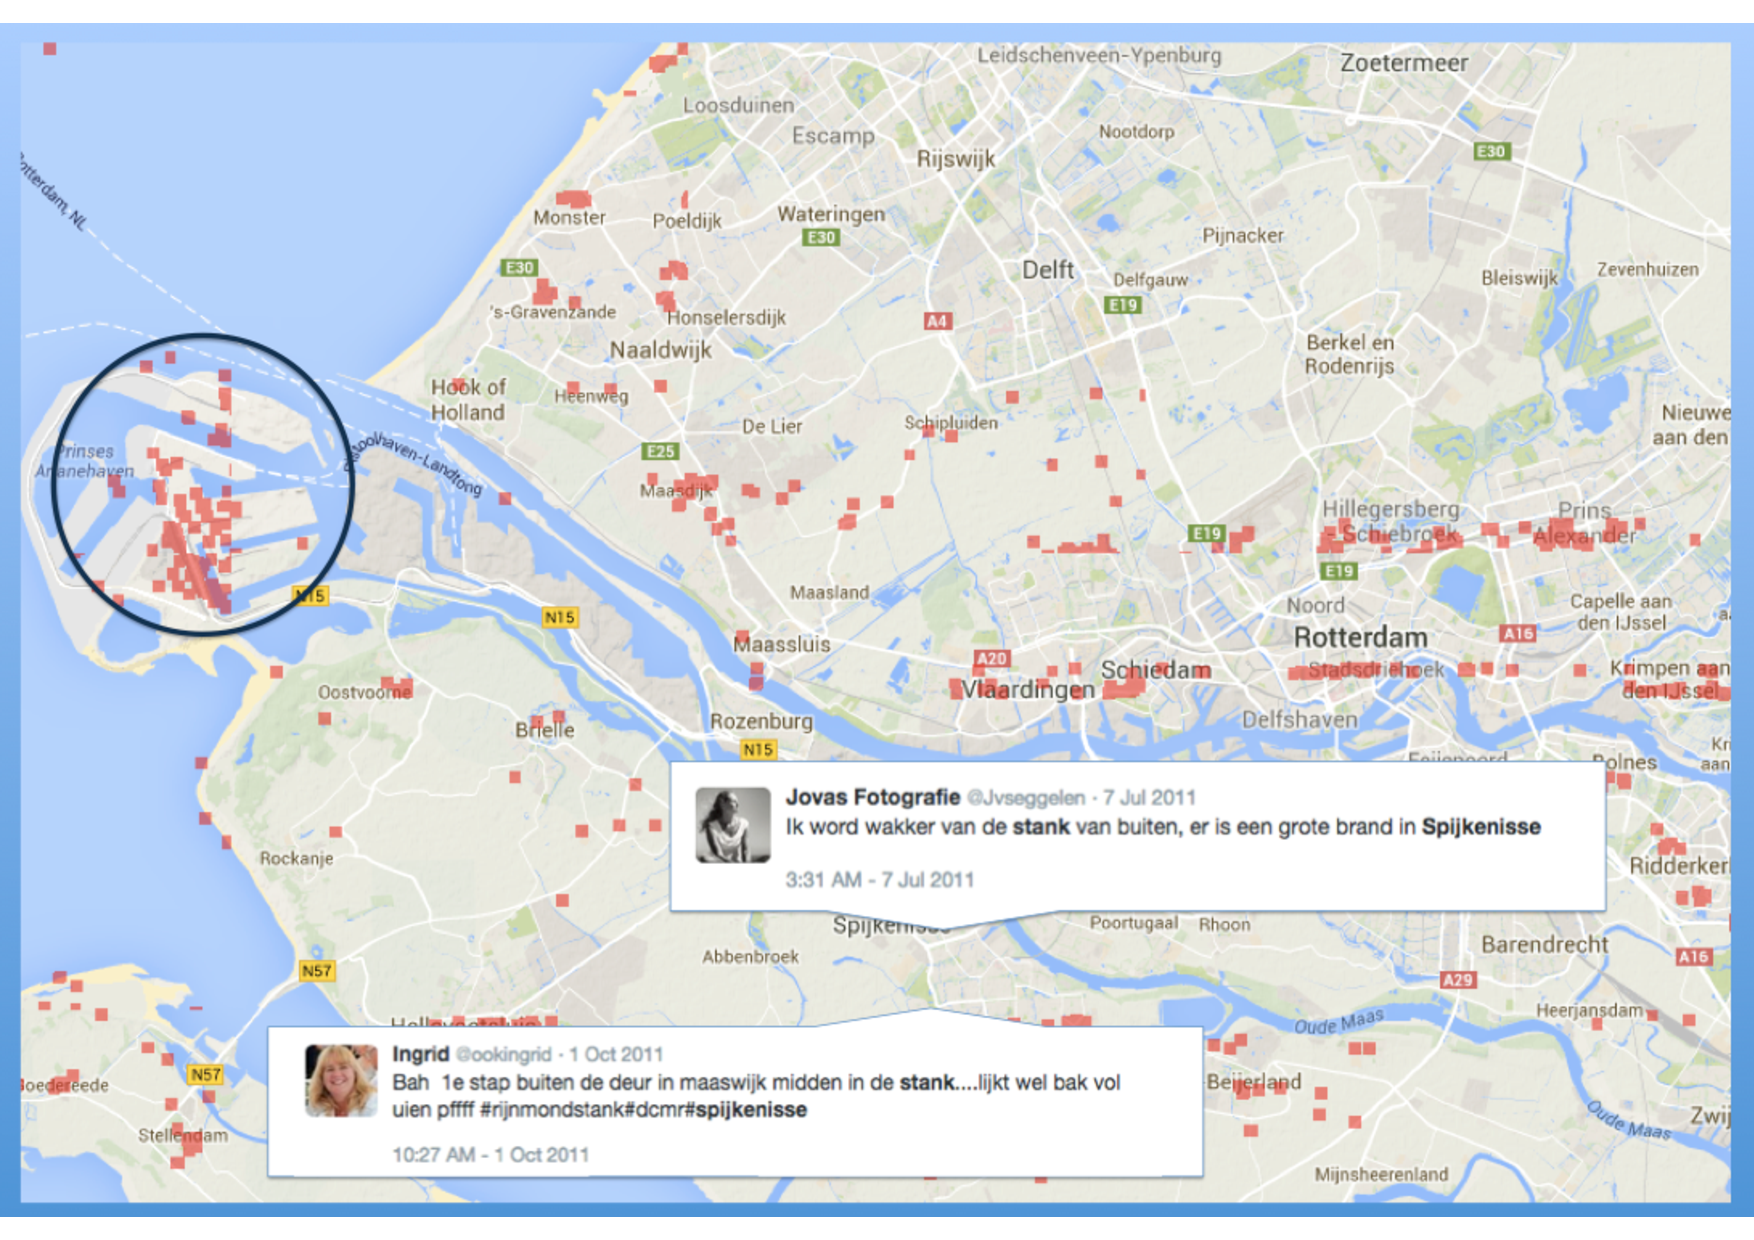
\includegraphics[width=4in]{Figures/DCMR-screenshot.pdf}
\caption{Tweets about excessive smells in the vicinity of the Rotterdam
harbor}
\label{fig:DCMR-screenshot}
\end{figure}

\paragraph{Nice to know}
The company Arcadis developed an application for the DCMR Milieudienst
Rijnmond based on the Stairwalk technology to investigate whether people
send tweets about unpleasant odors as a possible signal of danger (see
Figure~\ref{fig:DCMR-screenshot}). This turns out not to be the case,
probably because people think that nobody reads the tweets anyway. But if
people have the idea that their complaining tweets are read, then tweets
might be much more convenient than the reporting of unpleasant odors by
telephone.

\paragraph{This manual}

This manual explains how to use Stairwalker.  We first explain in
Section~\ref{sec:setup} how to install the required components in order to
have a basic running system.  We then explain in
Section~\ref{sec:deployment} how to add databases and different kinds of
datatypes to Geoserver, an open source server for sharing geospatial
data.\footnote{\url{http://geoserver.org}} It is explained how to show and
customize layers and views, but also how to adjust the system, for example,
how to add dimensions or use different dimension types such as median.
Finally, Section~\ref{sec:development} explains how to extend the system.

\paragraph{Acknowledgements}

This publication was supported by the Dutch national program COMMIT/.

\pagebreak
\section{Set Up}
\label{sec:setup}
In this section a detailed description is given about setting up all the
required peripheral programs to use Stairwalker.

\subsection{Database Setup}
Currently the Stairwalker program only works with the
PostgreSQL\footnote{PostgreSQL: \url{http://www.postgresql.org}} and
MonetDB\footnote{MonteDB: \url{http://www.monetdb.org}} database management
systems. This manual will only concern itself with PostgreSQL. Any further
reference to a database implies a PostgreSQL database.

In this section, we give a walk through explaining the steps needed to
setup PostgreSQL along with PostGIS\footnote{PostGIS:
\url{http://www.postgis.net}} and the database extension for
Stairwalker on an Ubuntu Linux operating system.

\subsubsection{PostgreSQL Database Manager Setup}
\label{sec:postgresql}

Installing Postgres on Linux should be straightforward. Search and install
the desired version of PostgreSQL. Below the commands used to search and
install version 9.1 of Postgres are shown.

\begin{enumerate}[noitemsep]
	\item \lstinline|aptitude search postgresql|
	\item \lstinline|apt-get install postgresql-9.1|
\end{enumerate}

For further information or if there are difficulties with the installation
more details can be found on the installation page of the
\href{http://www.postgresql.org/download/}{PostgreSQL website}.  

\subsubsection{PostgreSQL Configuration}

Once Postgres is installed on Linux two alterations will need to be made to
the configuration files so that the database can be accessed from outside
and by other users.

First, in the \lstinline|Postgresql.conf| file the
\lstinline|listen_addresses| need to be changed from \lstinline|localhost|
to \lstinline|all|. Assuming version 9.1 of Postgres this can be done as
follows.

\begin{enumerate}[noitemsep]
	\item \lstinline|cd /etc/postgresql/9.1/main|
	\item \lstinline|vi postgresql.conf|
	\item \textit{change} \lstinline|listen_addresses = `localhost'| \textit{to} \lstinline|listen_addresses = `*'|
	\item \textit{save and close}
\end{enumerate}

Secondly in the file \lstinline|pg_hba.conf| a line needs to be added to allow other users in Linux to access Postgres. This can be done as follows:

\begin{enumerate}[noitemsep,resume]
	\item \lstinline|vi pg_hba.conf|
	\item \textit{Add} \lstinline|host all all 0.0.0.0/0 password|
	\item \textit{save and close}
	\item \lstinline|/etc/init.d/postgresql restart|
\end{enumerate}

\noindent It should now be possible to create a database user and database
in PostgreSQL. In the sequel, we assume a database `\texttt{geonames}' is
created and used. More information about how this is done can be found on the
\href{http://www.postgresql.org/docs/manuals/}{\textsf{PostgreSQL manuals
webpage}}.

\subsubsection{PostGIS Configuration in PostgreSQL}
\label{sec:postgis}

The next step is to extend PostgreSQL with the PostGIS database expansion.
This again should be straightforward: first search for PostGIS and then
choose the version that goes with PostgreSQL to install. Note in order to do
the install root privileges are required. Below the commands to search and
install PostGIS for PostgreSQL-9.1 are shown.

\begin{enumerate}[noitemsep]
	\item \lstinline|aptitude search postgis|
	\item \lstinline|apt-get install postgresql-9.1-postgis|
\end{enumerate} 

\noindent More information about installing PostGIS can be found on the
\href{http://www.postgis.net/install}{\textsf{PostGIS website}}.

Once PostGIS is installed some extra configuration is required to add
PostGIS functionality to the used database (in our case
`\texttt{geonames}). This needs to be done as postgres user. The commands
are as follows.
\begin{enumerate}[noitemsep]
	\item \lstinline|createlang plpgsql geonames|
	\item \lstinline|psql -f `find/usr/share/postgresql/ -name postgis.sql -print' -d geonames|
	\item \lstinline|psql -f `find/usr/share/postgresql/ -name spatial_ref_sys.sql -print' -d geonames|
	\item \lstinline|psql -f `find/usr/share/postgresql/ -name postgis_comments.sql -print' -d geonames|
\end{enumerate}

\subsubsection{Serverside Stairwalker Extension in PostgreSQL}
\label{sec:serversideextension}

Stairwalker is a database extension written in C.  The extension has to be
compiled and installed in the PostgreSQL database. The extension can be
found in the directory
\lstinline|neogeo/pre-aggregate/src/db-extensions/postgres/pa_grid|.

The extension can be installed on Linux using the following commands.
\begin{enumerate}[noitemsep]
	\item \textit{go to the pa\_grid\ directory}
	\item \lstinline|make| \\ \textit{this creates the dynamic library}
	\item \lstinline|make install| \\ \textit{this installs the library in
		the PostgreSQL installation}
	\item \lstinline|make sql| \\ \textit{declare the module in the desired
		database}
\end{enumerate}

\noindent\textbf{Note} the extension has to be installed specifically for
the database which will be used for pre-aggregation. In the makefile (also
in the \lstinline|pa_grid| folder) there is a \lstinline|DATABASE| macro
which should be set to the desired database.

%\todo[inline, size=\small]{Installing the extension also requires root access. Why was this again?}


\subsection{Pre-Aggregate Database Table}
\begin{figure}[t]
\centering
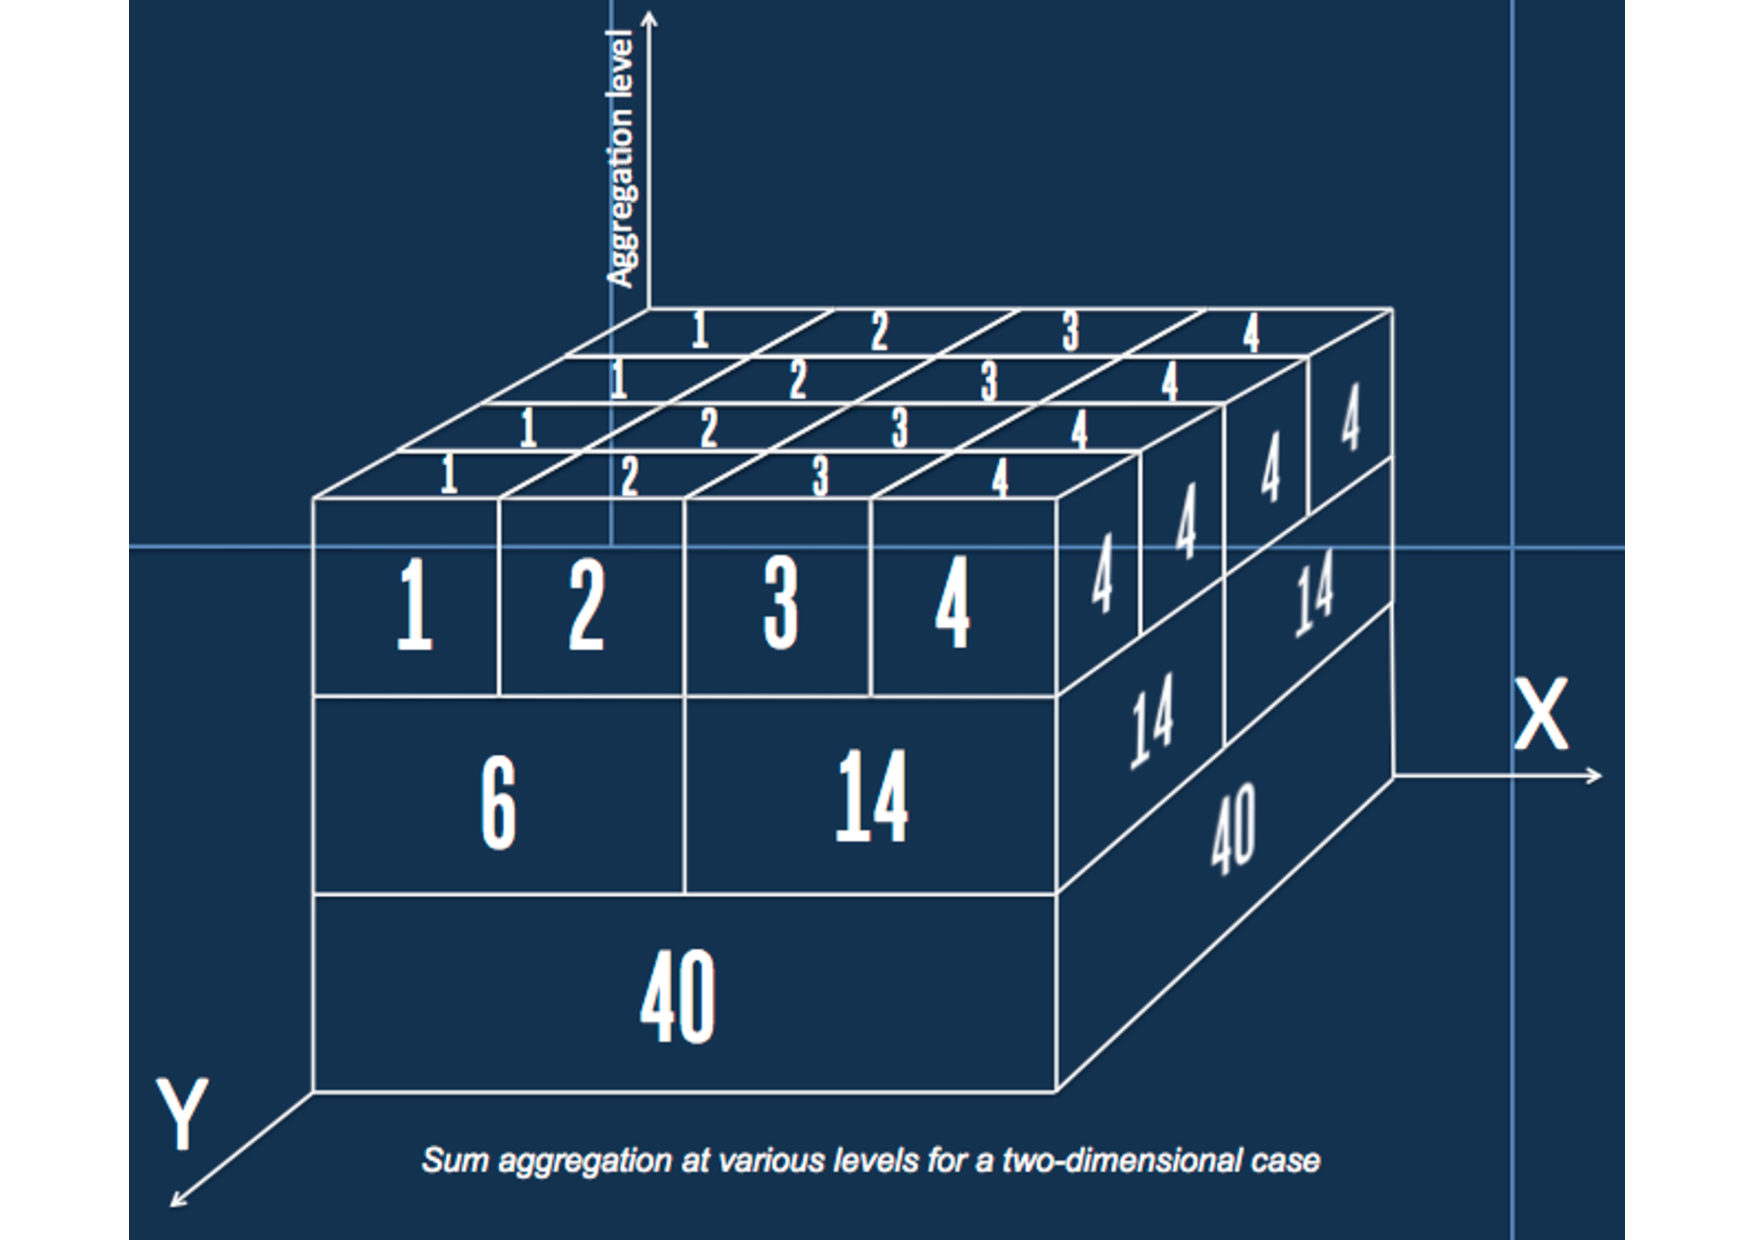
\includegraphics[width=4in]{Figures/grids.pdf}
\caption{Illustration of the grids concept}
\label{fig:grids}
\end{figure}


\subsubsection{Description of Process}

The indexing principle is as follows.  For the indexing of the data,
several grids are defined, with varying grid sizes. These grids can have
any number of dimensions. In the illustration of Figure~\ref{fig:grids}, we
show an example for the two-dimensional case. The third dimension in the
illustration depicts the aggregation grids at the various levels. For each
grid cell, the aggregation function is pre-calculated. Any suitable
aggregation function can be used, such as a summation, count,
maximum/minimum, etc. When a request comes in, the index returns the
pre-calculated values for all entirely included cells. The relatively small
amount of non-indexed values to complete the area is the calculated
on-the-fly, as illustrated on the right.

Concretely, take the dataset of tweets sent within the Netherlands (see
Figure~\ref{fig:NL-screenshot}. A pre-aggregation of this data, i.e.,
counts of tweets, could be in the following form. Dimensions are the x- and
y-coordinate dimensions. We set a highest granularity (zoom-level). The
pre-aggregate algorithm creates blocks bounded by the x- and y-coordinates
at the highest granularity and for all those blocks calculates the number
of tweets within the bounding box. Each subsequent layer is built up from
the previous layer. The final result is a dataset which contains the number
of tweets in a all bounding boxes at all levels of granularity.

\subsubsection{PreAggregate Tool}
\label{sec:preaggtool}

For off-line creation of the pre-aggregation index, a tool has been
developed. The tool can be found in the directory
\lstinline|neogeo/pre-aggregate-tools/|. To generate the binary tools from
source, the Appassembler plugin of Maven is used. Run the following command
to generate the tool.

\begin{lstlisting}
mvn package appassembler:assemble
\end{lstlisting}

After successful completion of this command, a new directory
\lstinline|appassembler| has been created in the \lstinline|target|
directory containing a \lstinline|repo| and a \lstinline|bin| directory.
The \lstinline|bin| directory contains the actual binaries of the tool (in
both Linux/Unix and Windows version) and the \lstinline|repo| directory
contains the tool dependencies. The tool should now be ready for use. An
example of how to compile and use the tool to create a pre-aggregation
index is given in \Fref{sec:examplePreAggIndex}.

The tool is used to create a pre-aggregate index for a table with
$\textit{n}$ dimensions and a measure/aggregate column. It uses with the
following commands:
\begin{lstlisting}[basicstyle=\small]
usage: create-pa-index
 -axistosplit <axis index>    index of axis to split
 -chunksize <size>            maximum chunk size after split
 -config <file>               PreAggregate XML config file
 -d,--database <dbname>       name of database
 -dbtype <postgresql|monetdb> type of database
 -h,--host <host>             database host name or ip address
 -help                        prints this help message
 -p,--port <port>             port number of the database
 -password <password>         database password
 -s,--schema <schema>         schema name in the database
 -u,--user <user>             database username
 -v,--verbose                 Enable verbose output logging
\end{lstlisting}
The tool depends on the \lstinline|PreAggregate.XML| config file which
is used to define the PreAggregate index by specifying the column to
aggregate, the type of aggregate that should done and the dimensions to
include. In the \lstinline|neogeo/pre-aggregate-tools/| directory a sample
configuration file is included.

%\todo[inline, size=\small]{How does this tool work nominal axis? More preprocessing may be required when first parsing words? Example london\_words or gender\_words}

See~\Fref{sec:PreAggregateDev} for more detail about creating a
pre-aggregate index not using the above tool.

Apart from creating a new pre-aggregate index table
\lstinline|<original-table-name>_pa|, pre-aggregation also creates/updates
two other tables: \lstinline|pre_aggregate| and
\lstinline|pre_aggregate_axis|. These two tables are support tables for the
aggregation. They contain information about which tables have been
aggregated and which axis have been used in pre-aggregation.

\subsubsection{Current Status Support of Axis Types}

The dimensions are referred to in the code as \lstinline|AggregateAxis|.
The axes have a base size and all layers above the base size are built up
by aggregating lower layer blocks. Currently the \lstinline|AggregateAxis|
can be split into two different subtypes. The first is a
\lstinline|MetricAxis| and the second is a \lstinline|NominalAxis|. Each
type will be briefly discussed below with examples of data types.

\paragraph{MetricAxis}
A \lstinline|MetricAxis| is the default axis type, it supports a continuous
data type. Examples of such data types are coordinates and time.

\paragraph{NominalAxis}
A \lstinline|NominalAxis| can be used for non-continuous dimensions. An
example for such a data type is a word filter. A \lstinline|NominalAxis|
can be used to split the data on occurrence of $x$ predefined words. 

For example, if a word filter \lstinline|{dog,cat,mouse,horse,NOFILTER}| is
used and a data block represents some text with the sentance
`\lstinline|it's raining cats and dogs|', then three splits would be made.
One on the word \lstinline|dog|, the second on \lstinline|cat| and the
third on \lstinline|NOFILTER|.

\subsubsection{Current Status Support of Aggregation Types}

Currently there are 4 different aggregation types which can be used. These
are discussed below. Note that there is an \lstinline|ALL| option which
returns all aggregate types in the pre-aggregate index. Furthermore these
types can be used to create other types such as average.

The current options are as follows:
\begin{enumerate}
\item \lstinline|ALL|: 	Returns all the aggregation types mentioned below.
\item \lstinline|COUNT|: Returns the count of items in an aggregate box.
\item \lstinline|SUM|: returns the sum of items in an agrregate box.
	For instance, a sum on the tweet length results in the total amount
	of characters tweeted in an aggregate box.
\item \lstinline|MIN|: Returns the lowest value in an aggregate box.
	With the example of tweet length, it returns the length of the shortest
	tweet in the aggregate box.
\item \lstinline|MAX|: Returns the highest value in an aggregate box.
	With the example of tweet length, it returns the longest tweet in the
	aggregate box.
\end{enumerate}

%\todo[inline, size=\small]{Small note, when using the pre-aggregate tool
%(created by Dennis) for the example \lstinline|ALL| was used as it crashed
%when using \lstinline|COUNT|, this should be looked into.}

It is important to choose the right type in order to get the desired
representation of the data.  To show the total number of tweets in a tile,
one should chose \lstinline|COUNT| as this will returns the total number of
data points in a tile. Whereas if one wants only the highest value in the
data (for example the highest building in an area) then \lstinline|MAX|
should be used.


\subsection{Tomcat Server Setup}
To visually display an aggregated dataset, a third party application is
used. This application is called GeoServer, GeoServer is an open source
server which can be used to display geospatial data. In order to run
GeoServer a web server is needed. 

Apache Tomcat\footnote{\url{http://tomcat.apache.org/}} has been used for
this purpose.  The use of Tomcat is not required for Stairwalker,
alternative options may also be used as long as it is possible to deploy
WAR files.  Whenever web hosting is mentioned in this manual it will be
assumed Tomcat is being used.

Information about setting up a Tomcat server can be found on the
\href{http://tomcat.apache.org/}{\textsf{Apache Tomcat website}}.

\label{sec:tomcat}

\subsection{Geoserver Deployment on Tomcat}
\subsubsection{Obtaining GeoServer and Aggregate Extension}

GeoServer\footnote{GeoServer: \url{http://www.geoserver.org}} is used to
visually display collected data pre-aggregated with the pre-aggregate
index. An extension has been written for
GeoServer which needs to be included in the web application. This is done
by including the JAR files of the extension in the \lstinline|WEB-INF| of
the GeoServer WAR file. A step by step guide is given below in
\Fref{sec:InstallExtension}. However before following these instructions
the necessary JAR and WAR files need to be obtained.

The GeoServer WAR file can be downloaded from the
\href{http://www.geoserver.org/download/}{\textsf{GeoServer website}}. The
custom Java extension files should be built using the source code. The
extension consists of the \lstinline|pre-aggregate| and
\lstinline|geoserver-ext| projects in the \lstinline|neogeo| project. Note
that first the JAR file of \lstinline|pre-aggregate| should be created as
it is a dependency of \lstinline|geoserver-ext|. The JARs can be built
using the command line or in an IDE such as Eclipse or Netbeans: using the
\lstinline|clean and build| command on a project in Netbeans should build
\lstinline|<project-name>-0.0.1-SNAPSHOT.jar| which can be found in the
\lstinline|target| directory of the respective project.

\subsubsection{Installing Extension}
\label{sec:InstallExtension}

The following instructions assume the geoserver extention files are located
in the directory \lstinline|/data/upload/| and the
\lstinline|geoserver.war| file is located in the directory
\mbox{\lstinline|/data/tmp/tmp_war|}. If this is not the case, the file
paths in the instructions below should be changed accordingly.

\noindent \textit{Unpack the WAR file}
\begin{enumerate}
	\item \lstinline|jar -xvf geoserver.war|
\end{enumerate}
\textit{Copy the JAR files of the extension into \lstinline|WEB-INF/lib| directory of the GeoServer unpacked WAR file}
\begin{enumerate}[noitemsep,resume]
	\item \lstinline|cp /data/upload/pre-aggregate-0.0.1-SNAPSHOT.jar /data/tmp/tmp_war/WEB-INF/lib|
	\item \lstinline|cp /data/upload/geoserver-ext-0.0.1-SNAPSHOT.jar /data/tmp/tmp_war/WEB-INF/lib|
\end{enumerate}
\textit{Recreate the GeoServer WAR file}
\begin{enumerate}[noitemsep,resume]
	\item \lstinline|jar -cvf geoserver.war META-INF/ WEB-INF/ index.html data/|
\end{enumerate}
The GeoServer WAR with the stairwalker extension should now be ready for
deployment.

\subsubsection{Deploying GeoServer}
\label{sec:geotomcat}

After the GeoServer WAR file has been repacked with the aggregate extension
included, it is ready to be deployed in a web server. \Fref{sec:tomcat}
describes how to set up a Tomcat web server. Once the server is
running, it can be accessed locally with
\href{http://localhost:8080/}{\lstinline|http://localhost:8080/|} assuming
default installation configuration were used, otherwise the port number
might be different. In the case that the Tomcat server is installed on a
different machine, the web server can be accessed by replacing
\lstinline|localhost| with the name or IP address of that machine.

From the Tomcat homepage, it should be possible to access the Tomcat manager
webapp. With the default setup it should be possible to login with the
following credentials:\\
\indent \textbf{username:} manager \\
\indent \textbf{password:} tcmanager \\

In the Tomcat manager webapp under the \lstinline|deploy| section, it is
possible to upload a WAR file to be deployed. Select the repacked WAR file
from \Fref{sec:InstallExtension} and deploy the application. Once the
application is deployed it will be displayed in the \lstinline|application|
section of the Tomcat manager webapp. From there, it is possible to follow
the path given for the GeoServer application or, if the default
configuration was used to go to
\mbox{\lstinline|http://<Tomcat-IPaddress>:8080/geoserver/web/|}.

\label{sec:geoserverinstall}


\pagebreak
\section{Deployment}
\label{sec:deployment}
This section gives a detailed description of how to import an
aggregated database table into GeoServer to get a visual representation of
the dataset. First instructions will be given on how to link the database
table to GeoServer. Next, creating styles and layers for data representation
will be discussed. The final section discusses how to view the data
using GeoServer.  For this section it is assumed that all the initial
preparation discussed in \Fref{sec:setup} has been completed.

GeoServer should already be deployed on a web server (see
\Fref{sec:geotomcat}), and can then be accessed with
\lstinline|http://<Tomcat-IPaddress>:8080/geoserver/web/|. It is required
to login in to the GeoServer web administration interface. When using the
default setup of GeoServer the login credentials are: \\
\indent \textbf{username:} admin \\
\indent \textbf{password:} geoserver

\noindent A concrete example of how to fully deploy a pre-aggregated index
can be found in \Fref{sec:exampleGeoServer}.

\subsection{Add Source}
\label{sec:addingsource}
%Once the webapplication has logged in, then start by adding the source of the database. 
%\begin{enumerate}
%	\item On the left side there should be a menu with all kinds of options, but in order to add a source, go to Configuration $\rightarrow$ Sources. 
%	\item At the top there should be an add source button. 
%	\item Now under vectortypes there should be a list of types. Select what kind of source you want to add. In order to get the Stairwalker program running there should be a NeoGeo Aggregate - NeoGeo aggregation index query. If this is not the case something went wrong with deploying the geoserver and the last steps in this manual should be done again. 
%	\item If it is here, click on it and a new menu will open. A new screen should open where all information for your source has to be filled in. There is also an option on what aggregation type the program should use, this should have been defined before so use what has been used before (count/sum/minimum/maximum). 
%	\item Once everything is filled in all, the source should have been added to the Geoserver. This can be checked by going to sources again and then it should display the source that has just been added.
%\end{enumerate}

Once logged in to the web administration interface, it is possible to add a
new data store to GeoServer. Below are instructions of how to add a new
\lstinline|NeoGeo Aggregate| vector data source which contains the
aggregate index created in \Fref{sec:preaggtool} to the stores in
GeoServer.

\begin{enumerate}
	\item Navigate to \lstinline|Stores| by clicking on \lstinline|Stores| link under the \lstinline|Data| section in the navigator on the left hand side of the web administration interface homepage.
	\item On the \lstinline|Stores| page select the option \lstinline|Add new Store| located at the top of the page. This leads to a page titled \lstinline|New Store chooser|.
	\item In the list of \lstinline|Vector Data Sources| the option \lstinline|NeoGeo Aggregate| should be present, choose this format for the data source.  
\end{enumerate}

\noindent If the option \lstinline|NeoGeo Aggregate| is not available, it
means the GeoServer extension from \Fref{sec:InstallExtension} was not done
correctly.

\begin{enumerate}[resume]
	\item Clicking \lstinline|NeoGeo Aggregate| will open a new page titled \lstinline|New Vector Data Source| in which several fields have to be filled out, explanation of mandatory fields can be found in the list below.
	\item For an express setup the fields which have already been filled can remain the same.
	\item Once all the required fields are filled, click the \lstinline|Save| button.
	\item A new \lstinline|NeoGeo Aggregate| source is now created and can be viewed and edited in \lstinline|Sources|.
	\item After saving, GeoServer opens the page \lstinline|New Layer| on which new layers can be created using the \lstinline|Data Source|. How this is done is discussed in \Fref{sec:addinglayers}.
\end{enumerate}

\noindent Below a list is presented with all mandatory fields on the
\lstinline|New Vector Data Source| page with explanation.

\begin{itemize}\label{list:manditory}
	\item \textbf{Data Source Name} - An arbitrary name which will be assigned to the store.
	\item \textbf{Database type} - The type of underlying database, either PostgreSQL or MonetDB.
	\item \textbf{Hostname} - Hostname of the database server where the aggregation index is maintained.
	\item \textbf{Port} - Port number of the database.
	\item \textbf{Schema} - Name of the schema where the aggregation index is maintained.
	\item \textbf{database} - Name of the database where the aggregation index is maintained.
	\item \textbf{Username} - Username of the used database.
	\item \textbf{Password} - Password of the used database.
	\item \textbf{xSize, ySize, timeSize} - Specifies the dimensions of the grid which is created for every view of the map to calculate the aggregates per cell. The higher the number of cells the more detailed the information. \\
	%\todo[inline, size=\small]{Are the xSize, ySize, timeSize dimensions not already set in the source? What happens when timeSize $> 1$?}
	\item \textbf{count, sum, minimum, maximum} - Select the boxes of the
	aggregates which will be used in the visualization. Note that from these basic aggregates more aggregates such as mean can can be derived.
	\item \textbf{Enable server-side Stairwalker} - Selecting this causes the data source to rely on the use of the database plugins to use the Pre-Aggregate index. For performance reasons it is highly recommended to use this option. See \Fref{sec:serversideextension} for more details.
%	\todo[inline, size=\small]{The Enable server-side Stairwalker ooption is no longer available? Remove?}
	\item \textbf{Enable query logging} - Selecting this will turn on the logging of all Pre-Aggregate queries into a separate table called \lstinline|pre_aggregate_logging|.
\end{itemize}

\pagebreak

\subsection{Setup Style}
\label{sec:addingstyle}
%The next step is to make a style in which you want your data to be shown. A style has to be made in SLD/XML, there are a lot of options which can be used to make a style. First navigate to the style tab, Configuration $\rightarrow$ Style here you can add a new style with the button on top. Here you need to add your code (or file) for your style.
%\newline
%\newline http://docs.geoserver.org/2.5.x/en/user/styling/sld-cookbook/index.html contains a lot of information regarding styles, it is a lot of trial and error to get a nice working style. The next few steps however should give a short setup on how to start making your own style.
%\begin{enumerate}
%	\item Decide what data should be shown, in our example we’re using the count of the aggregated data.
%	\item Decide what kind of representation should be used, you can either use Polygonsymbolizer, pointsymbolizer or linesymbolizer. All of these have their own advantages and disadvantages, incase it isn't clear what to use, start off with a Polygonsymbolizer.
%	\item Add all filters, for instance if the data should how a lighter color if the amount is lower. Or make a tile red once the data exceed a certain maximum (for instance if there were too many orders in a timerange).
%	\item Add colors to the layers representing it better and giving it a nice layout.
%	\item Make sure the positioning of the label and all filters are working.
%	\item Finish the layer by adding the last details (Halo behind the text for example).
%\end{enumerate}
%
%This is just a basic manual on how to add a style, for more information or more explanation on how to make a style, check out the development chapter in this manual. In that section there are far more details on how to make a style.
%

In GeoServer, styles are used to render, or make available, geospatial data.
Styles are used to visually represent the aggregation index which is
represented in a layer. In GeoServer layers are written in Styled Layer
Descriptor (SLD) which is a subset of XML. GeoServer comes setup with
several different styles, however, to get the most out of the dataset it is
best to develop a style specific to the layer which represents that data.

In this section only instructions on how to add new styles to GeoServer are
given. For information on how to edit styles, see \Fref{sec:visualization}
or the GeoServer user
manual\footnote{\url{http://docs.geoserver.org/stable/en/user/styling/index.html\#styling}}
which gives an in depth guide on developing styles.

\begin{enumerate}
	\item Navigate to \lstinline|Styles| by clicking on the \lstinline|Styles| link under the \lstinline|Data| section in the navigator on the left hand side of the web administration interface homepage.
	\item On the \lstinline|Styles| page select the option \lstinline|Add a new style| located at the top of the page.
	\item A new page titled \lstinline|New Style| should open. There are now two possibilities, either a new style can be developed completely in the browser or a SLD file can be imported.
	\item To import an already created SLD file scroll to the bottom of the page and press the \lstinline|Choose File| button.
	\item Select the style which should be imported and then press \lstinline|Upload...| in the browser.
	\item This fills in the \lstinline|Name| field with the name of the file and the SLD editor with the content of the file.
	\item It is possible to check the syntax of the SLD code by pressing the \lstinline|Validate| button at the bottom of the page. At the top the page GeoServer will give feedback on the SLD code, either error messages or a no validation errors message.
	\item Finally the style can be saved by pressing the \lstinline|Submit| button at the bottom of the page.
\end{enumerate}
%\todo[inline, size=\small]{We should maybe mention something about the workspace? What does \lstinline|nurc| represent? It is even important to choose a workspace?}


\subsection{Adding Layer}
\label{sec:addinglayers}
%Now we have a source and have a style to use, it is time to setup a layer to display this style. 
%\begin{enumerate}
%	\item Go to Configuration $\rightarrow$ Layers and press the button on top, A drop down menu should appear in where the database has to be selected.  Once a database has been selected there should be a couple of options of which data should be displayed.
%	\item Select the data you want and press Publish. Fill in all these fields in order to get the layer to work. Important are the projections. In our layers we use Projection of Source, EPSG:4326, and Given Projection, EPSG:3857. And set handling of the projection to use the given projection. Then for Boundary Rectangles let them be calculated based on sourceprojection. And then all fields should be filled in, do not press save yet however. 
%	\item On top select publish. Select the style which should display your data, select the style that has been made in the last step here. If there is no style that can be displayed, something went wrong and the last steps should be repeated.
%	\item Once this is done press save and the layer should be added.
%\end{enumerate}

In GeoServer, a layer refers to raster or vector data that contains
geographic features. Layers represent each feature (axis in the
pre-aggregate index) of a dataset that needs to be represented. All layers
much have a source of the data which in this case was setup in
\Fref{sec:addingsource}. More information about layers can be found in the
\href{http://docs.geoserver.org/stable/en/user/webadmin/data/layers.html}{GeoServer
User Manual}. 

Creating a layer for a pre-aggregate index dataset can be done as follows:

\begin{enumerate}
	\item Navigate to \lstinline|Layers| by clicking on the \lstinline|Layers| link under the \lstinline|Data| section in the navigator on the left hand side of the web administration interface homepage.
	\item On the \lstinline|Layers| page select the option \lstinline|Add a new resource| located at the top of the page.
	\item This leads to a new page where the \lstinline|Store| which contains the layer needs be chosen from a drop-down list. If there are no \lstinline|Store|s available make sure one was added, see \Fref{sec:addingsource} 
	\item Choose the \lstinline|Store| in which the aggregation index is stored.
	\item Once a \lstinline|Store| is selected a list of resources contained in the \lstinline|Store| is given. These resources are the different aggregated indexes in the database which was linked to a \lstinline|Store| in \Fref{sec:addingsource}.
	\item Select the pre-aggregate index which should be visualized in a layer by clicking the \lstinline|Publish| link corresponding to the \lstinline|Layer name| of the aggregate index.
\end{enumerate}

\noindent At this point a layer has been selected to be published. This
layer will be a visual representation of the data from the aggregation
index created in \Fref{sec:preaggtool}. In order to make sure the correct
geographical location is used in GeoServer and to give the layer a fitting
style the following steps have to be taken in on the \lstinline|Edit Layer|
page.

\begin{enumerate}[resume]
	\item In the \lstinline|Data| tab the following sections and fields should be filled in.
	\begin{enumerate}
		\item In the \lstinline|Basic Resource Info| there are some labeling fields. Standard the \lstinline|Name| and \lstinline|Title| are \lstinline|<aggregation-index-tablename>| followed by \lstinline|___myAggregate|. These can both changed to whatever is desired. However make sure the that the \lstinline|Enabled| box is ticked in this section.
		\item In the \lstinline|Coordinate Reference Systems| section there are three fields.
			\begin{enumerate}
				\item \lstinline|Native SRS| should be \lstinline|EPSG:4326|.
				\item \lstinline|Declared SRS| should be \lstinline|ESPG:3857|. This coordinate system is used since it is what is usually used for tile based map representation.
				\item \lstinline|SRS handling| should be \lstinline|Reproject native to declared|.
			\end{enumerate}
		\item In the \lstinline|Bounding Boxes| the coordinates corresponding to the data from the aggregation index is calculated for GeoServer. For \lstinline|Native Bounding Box| click \lstinline|Compute from data| and for \lstinline|Lat/Lon Bounding Box| click \lstinline|Compute from native bounds|.
		\item All other sections in this tab are of little importance in a basic deployment.
	\end{enumerate}
	%Some very ugly things happen with \lstinline here to make things fit nicely on the page. Sorry =(
	\item Next in the \lstinline|Publishing| tab a style can be added to the layer, the default style of a layer is \lstinline|polygon|. In the section \lstinline|WMS Settings| the field \lstinline|Default| \lstinline|Style| can be changed by selecting the desired style from the drop-down menu. For more about styles and creating styles see \Fref{sec:addingstyle} and \Fref{sec:visualization}.
\end{enumerate}

\noindent If the aggregation index does not contain a time dimension the
setup of the layer is now complete and can be saved. However if the
aggregation index does have a time dimension some additional adjustments
need to be made which are described below.

\begin{enumerate}[resume]
	\item Select the \lstinline|Dimensions| tab.
	\begin{enumerate}
		\item Enable the the \lstinline|Time| dimension.
		\item As \lstinline|Attribute| select \lstinline|starttime|.
		\item Do not set an \lstinline|End Attribute|.
		\item As \lstinline|Presentation| select \lstinline|Continuous interval|.
	\end{enumerate}
	\item Save the layer.
\end{enumerate}

The layer which represents the dataset with a style created in
\Fref{sec:addingstyle} has now been created and is ready for use. A layer
can be edited once it has been created so if changes need to be made a new
layer should not be created. \Fref{sec:previewlayer} shows how to preview a
layer and \Fref{sec:clientsidedev} discusses how to use a GeoServer layer
with OpenLayers\footnote{\url{http://openlayers.org/}} to a geospacial
visualization of the data on a web page.


\subsection{Viewing and Using Layer}
\label{sec:previewlayer}
%Now in order to see the layer go to view, here it should display the layer that has been made (with the added name) with a drop-down menu. Select PNG/JPEG or something similar to show a basecase of the data. A new window should open and here it should show your data in a weird graph. If this is not the case, its likely a mistake in the style. It is also possible to adjust your view in the images by adding a VIEWPARAM to the url. To do so just add: \&VIEWPARAMS=$<$Type$>$:$<$Value$>$ to the url and the image should change.

In GeoServer it is possible to get a preview of layer such as the one
created in \Fref{sec:addinglayers}. Previewing a layer can be done as
follows:

\begin{enumerate}
	\item Navigate to \lstinline|Layer Preview| by clicking \lstinline|Layer Preview| link under the \lstinline|Data| section in the navigator on the left hand side of the web administration interface homepage.
	\item The \lstinline|Layer Preview| page will have a list of all configured layers with can be previewed in various formats.
	\item Locate the layer which should be shown and from the \lstinline|All Formats| column choice any \lstinline|WMS| format.
	\item After selecting a format to view the layer a new page will open with a visual representation of the top most layer of dataset.
\end{enumerate}

Note that other preview formats should also be possible. For example it is
possible to use the OpenLayers preview format which allows one to navigate
the geospatial data. In section \Fref{sec:clientsidedev} OpenLayers will
also be used to visualize the dataset on a web page. One drawback is that
for every movement in the preview a new query has to be calculated. When
server side stairwalker (\Fref{sec:serversideextension}) is not setup
calculating can be time consuming. Therefore during development of the
pre-aggregation index and testing it is adviced to use a static preview and
only once everything works as desired to use a dynamic preview.

If the layer contains a nominal axis it is possible to alter the value of
the nominal with which the data is filtered. This is done by adding a
parameter in the request made to the GeoServer extension. By extending the
\lstinline|HTML| request sent to GeoServer with
\lstinline|&VIEWPARAMS=<TYPE>:<VALUE>;| the nominal axis filter is used.
Currently the extension only supports the nominal type \lstinline|keyword|.
If the pre-aggregate index was created using a nominal axis (splitting on
\lstinline|VALUE|s) then using \lstinline|&VIEWPARAMS| will split the
visualization on a give \lstinline|VALUE|. \lstinline|&VIEWPARAMS| can
accept more \lstinline|<TYPE>:<VALUE>;| tuples, however parsing type will
need to be extended on in the code. For more information see
\Fref{sec:filtering}.

It may be that a preview fails to load, this can be due to two reasons. The
first is an error in the style, in this case the style needs to be tested
which can be done by validating the style in GeoServer. For more
information about styles see \Fref{sec:visualization}. The second reason is
an error is creating an SQL query for the pre-aggregated index. If no
mistakes where made during setup and in creating a pre-aggregate index
there will be a need to dive into the code where detailed logging is done.

%\todo[inline, size=\small]{This would be a good point to reference the
%logging done in the code however i cannot find where this log file is
%located, debugging is also possible using the console in an IDE.}




\pagebreak
\section{Development}
\label{sec:development}
\subsection{Code Development}
\label{sec:PreAggregateDev}
In this section, some pointers will be given to important sections of code
in terms of processing pre-aggregate indexes which are used by the
GeoServer extension.

%MvK: ???
%During the development of Stairwalker, the developers project of GeoServer,
%the source code used is available to download on the GeoServer website.
Using the source code GeoServer and running it from an IDE, provides useful
information for troubleshooting, as logging information is printed directly
to the console, and for constant redeployment a new WAR file does not have
to be remade every time. The source code of the Stairwalker project is
available on GitHib\footnote{\url{https://github.com/utwente-db/neogeo}}.
The two important packages from this project are \lstinline|geoserver-ext|
and \lstinline|pre-aggregate|. The first is the extension used in GeoServer
to handle pre-aggregation indexes as data sources and the second is the
package which is used to create the pre-aggregate index.

\subsubsection{Creating Pre-Aggregate Index from Source}

%\todo[inline, size=\small]{This subsection is still superficial in some aspects. I am unsure how extensive an explanation is required here and if it is even necessary.}

Creating a pre-aggregate index can be done using a tool as shown in
\Fref{sec:preaggtool}. It is also possible to create a new method in the
\lstinline|Test.java| of \lstinline|pre-aggregate| in which the steps for
creating the pre-agggregation index can be done manually. In the
\lstinline|main| of this class configuration file
\lstinline|database.properties| is read, which contains login information
about the database which contains the dataset, and connection is made to
said database. Next a pre-aggregate index is made using the custom made
method which describes the pre-aggregation. How to set up such a method is
described in this subsection.

Firstly for each axis on which the dataset will be split an
\lstinline|AggregateAxis| variable will be defined. Next these variables
should be initiated with a axis type (\lstinline|metric| or
\lstinline|nominal|), in the case of \lstinline|nominal| also a word list
(which contains the words on which the dataset will be split) should be
created. The constructors of both axis types are as follows:

\begin{lstlisting}
public MetricAxis(String columnExpression,
	String type, Object BASEBLOCKSIZE, short N);
	
public NominalAxis(String word_collection_column, 
	String word_index_column, String wordlist_str, 
	String name);
\end{lstlisting}

Once all axes have been initialized, an array containing all axes should be
created which will be used as input for the \lstinline|PreAggregate|
variable created in the next. The next step is to create a pre-aggregate
index by creating and initiating a \lstinline|PreAggregate| variable. The
constructor of \lstinline|PreAggregate| is as follows:

\begin{lstlisting}
public PreAggregate(Connection c, String schema,
	String table, String override_name,
	String label, AggregateAxis axis[],
	String aggregateColumn, String aggregateType,
	int aggregateMask, int axisToSplit,
	long chunkSize, Object[][] newRange);
\end{lstlisting}

Afterwards the connection to the database should be closed. A method
containing these components is created and it can be statically run in the
main. Note that with the \lstinline|NominalAxis|, some prepossessing maybe
required on the dataset. In order to do this, the help method
\lstinline|tagWordIds2Table| is used. On \lstinline|NominalAxis| the
\lstinline|tagWordIds2Table| method has the following arguments:

\begin{lstlisting}
public void tagWordIds2Table(Connection c, 
		String schema, String org_table, 
		String new_table);
\end{lstlisting}

\subsubsection{Filtering Words for Nominal Axis}
\label{sec:filtering}

In the package \lstinline|geoserver-ext|, specifically the class
\lstinline|AggregationFeatureSource| creates the SQL query which requests
data from the pre-aggregated index for which GeoServer is built. If the
pre-aggregated index contains a \lstinline|Nominal| axis, then it is
possible to pass along words to filter the axis in GeoServer using
\lstinline|VIEWPARAMS| (see \Fref{sec:previewlayer}). In order to include
this filter parameter, the method \lstinline|getReaderInternal| and possibly
\lstinline|reformulateQuery| should be extended.

In the method \lstinline|getReaderInternal|, the layer request sent to
GeoServer is parsed including the \lstinline|VIEWPARAMS|, so a variable
should be created in the method which matches the word which should be
filtered given by \lstinline|<TYPE>:<VALUE>|. This variable can then be
passed to the \lstinline|reformulateQuery| method. It is then possible in
\lstinline|reformulateQuery| for a specific \lstinline|AggregateAxis| to
split on the variable passed along in \lstinline|getReaderInternal|.

\pagebreak

\subsection{Geoserver Visualization}
\label{sec:visualization}
This section discusses most of the possibilities that GeoServer has to
offer when it comes to the visualization of the data. The GeoServer manual
has some information on this subject, which can be found on:
\url{http://docs.geoserver.org/2.5.x/en/user/styling/sld-reference/index.html}.

In the following, more information on what the differences are between the
certain options and some ways to implement these options. This section uses
some of the examples used in our demo to give some more insight what can be
done and hopefully making it easier to realize what is desired. Most
information can be found on the website, below a discussion is given on
what types are best used when, but also some more information on how to
make them work properly.

\subsubsection{Symbolizers}

In SLD, there are three different symbolizers, a linesymbolizer, a
pointsymbolizer and a polygonsymbolizer. A pointsymbolizer is used when the
data that has to be represented is best shown as points. It does exactly
what it says, you'll get a map with points on it and each point will
represent a data-object from your dataset. This symbolizer can be really
handy in certain situations. For example when you want to show all
locations where a rare species of a bird has been found, it will show a map
with all points where a bird has been reported.

A linesymbolizer is used when the data that has to be displayed is best
shown in lines. This symbolizer is best used to display roads for example.
It isn't a symbolizer that can be used to represent data very well, but it
is more used for pre-defined data, such as rivers, roads etc.

A polygonsymbolizer is used when the data that you want to represent has to
be displayed in two-dimensional objects. There are many possibilities in a
polygonsymbolizer. It is possible to make a simple square but it also has
the option to make circles or triangles. It is one of the most commonly
used symbolizers.  A good example where a polygonsymbolizer is used, is to
display the amount of people living in cities. This can be done with a
circle polygon and that the circle will get bigger when more people live in
a city.

\subsubsection{Filters}

Filters are the most important function when it comes to making a custom
style. A filter is basically the basis of a fancy layer. What a filter does
is that it makes a ruling and if that ruling is met, the color, labeling
etc will be done. In SLD, it is possible to have an unlimited amount of
filters so the possibilities are many. The following filter expression
can be used:

\begin{itemize}
	\item \lstinline|$<$PropertyIsEqualTo$>$|
	\item \lstinline|$<$PropertyIsNotEqualTo$>$|
	\item \lstinline|$<$PropertyIsLessThan$>$|
	\item \lstinline|$<$PropertyIsLessThanOrEqualTo$>$|
	\item \lstinline|$<$PropertyIsGreaterThan$>$|
	\item \lstinline|$<$PropertyIsGreaterThanOrEqualTo$>$|
\end{itemize}
An example on how a single filter can be used is the following:
\begin{lstlisting}
<ogc:Filter>
  <ogc:PropertyIsLessThan>
    <ogc:PropertyName>testvalue</ogc:PropertyName>
    <ogc:Literal>200</ogc:Literal>
  </ogc:PropertyIsLessThan>
</ogc:Filter>
\end{lstlisting}

This example tests if \lstinline|testvalue| is less than \lstinline|200|.
If this is the case, one can specify what the filter should do. Below is
the complete example that does something with this filters.

\begin{lstlisting}
<Rule>
  <Name>SmallPop</Name>
  <Title>Less Than 100</Title>
  <ogc:Filter>
    <ogc:PropertyIsLessThan>
      <ogc:PropertyName>testvalue</ogc:PropertyName>
      <ogc:Literal>100</ogc:Literal>
    </ogc:PropertyIsLessThan>
  </ogc:Filter>
  <PolygonSymbolizer>
    <Fill>
      <CssParameter name="fill">#38FF19
      </CssParameter>
      <CssParameter name="fill-opacity">1.0
      </CssParameter>
    </Fill>
    <Stroke>
      <CssParameter name="stroke">#000000
      </CssParameter>
      <CssParameter name="stroke-width">1.0
      </CssParameter>
    </Stroke>
  </PolygonSymbolizer>
</Rule>
\end{lstlisting}

What this example does is that if the \lstinline|testvalue| is below
\lstinline|100|, it will fill a polygon with the color:
\lstinline|#38FF19|. If this is not the case, it will go to the next rule
(if there is one; otherwise it does nothing). The image shows a graph of
the implementation we made for our data. The image has different kind of
colors for the amount of data in a tile. If the amount is high, the color
will become more red, and if there is little data, the tile will be green.

\subsubsection{Additional Options}

GeoGerver SLD has a lot of options when it comes to customizing the data
display that you've made. Below are some of the important features that are
commonly used in GeoServer.

\textbf{Halo:} A halo gives a glow behind the current label. It should
always be used in a textsymbolizer, since this is the only place where you
can add a halo. To use a halo is very simple: you include
\lstinline|<Halo></Halo>| and in between it is possible to add
\lstinline|<Radius>| and \lstinline|<Fill>|. For more information on how to
use a \lstinline|<Fill>| we refer to the GeoServer SLD cookbook.

\textbf{Anchorpoint:} An anchor point is a handy tool to place your label
in a possible position. It is used as shown below. Important to note is
that you can set where the anchor point is (for example, above the point)
and that you can move it based on the anchor point, for instance make it go
all the way to left (negative X placement) or all the way to the right
(positive X placement)
\begin{lstlisting}
<PointPlacement>
  <AnchorPoint>
    <AnchorPointX>0.5</AnchorPointX>
    <AnchorPointY>0.0</AnchorPointY>
  </AnchorPoint>
  <Displacement>
    <DisplacementX>0</DisplacementX>
    <DisplacementY>25</DisplacementY>
  </Displacement>
  <Rotation>-45</Rotation>
</PointPlacement>
\end{lstlisting}

\textbf{Opacity:} Opacity is the transparency of either a label, point,
polygon or line. It can be used to paint layers over each other (setting
Opacity to 0). It is often used in cases where multiple data sets have to be
displayed in the same tile (used in our example as well). The way you use
it is the following:
\begin{lstlisting}
<Opacity>0.3</Opacity>
\end{lstlisting}

\textbf{Rotation:} Rotation is the function that is used to turn shapes and
labels in SLD. It is handy if you want to turn tiles or make labels line up
with lines better. The way to use it is simply in the section that has to
be rotated just add the following code:
\lstinline|<Rotation>-45</Rotation>| for a negative 45 degree turn.

\textbf{Graphic Fill:} A graphic fill is used in case a picture/image has
to be shown in a layer. It has a lot of possibilities since every
picture/image can be added in this way. The implementation is a little
more complex; below is an example of a graphic fill. 
\begin{lstlisting}
<FeatureTypeStyle>
  <Rule>
    <PolygonSymbolizer>
      <Fill>
        <GraphicFill>
          <Graphic>
            <ExternalGraphic>
              <OnlineResource
              xlink:type="simple"
              xlink:href="colorblocks.png" />
              <Format>image/png</Format>
            </ExternalGraphic>
            <Size>93</Size>
          </Graphic>
        </GraphicFill>
      </Fill>
    </PolygonSymbolizer>
  </Rule>
</FeatureTypeStyle>
\end{lstlisting}
More options and information can be found in the SLD cookbook on the
GeoServer website. This section was meant to give some more insight about 
commonly used functions.
  

\pagebreak

% Empty:
%\subsection{Client Side Development}
%\label{sec:clientsidedev}
%\todo[inline]{Here Mathijs will write a subsection on what is possible in terms of client side development with respect to the stairwalker project.}


\pagebreak
\section{Running Example}
In this section, a concrete example is given to show how to use Stairwalker.
The example runs from creating a pre-aggregation index from a given dataset
to geospacially representing the data using GeoServer. For the example, a
dataset is provided in terms of a .csv file. It concerns an exported list
of tweets sent in the UK and which carry a GPS coordinate.

The result expected in this example can be seen in \Fref{fig:result}.
Different colors represent the number of tweets in a region. The result
only shows the highest granularity. Each tile shows how many tweets are
sent from a location within the tile.  If this layer is combined with a
map, it would be clear that the region of this figure is directly above the
UK.

\subsection{Requirements}
Before showing how to create the given example, all necessary installations
should have been completed and the required files obtained.
The following programs should be installed:
\begin{enumerate}
	\item PostgreSQL (\Fref{sec:postgresql})
	\item PosgGIS for a PostgreSQL database (\Fref{sec:postgis})
	\item Tomcat or another web service server (\Fref{sec:tomcat})
	\item GeoServer with extension (\Fref{sec:geoserverinstall})
\end{enumerate}
Also the following files should be at the ready:\footnote{The files can be
found in the \lstinline|RunningExample| directory in the same Git as this
manual.}
\begin{enumerate}
	\item The tool to make a pre-aggregate index: Pre-Aggregate-Index tool
		(\Fref{sec:preaggtool})
	\item Configuration file for the tool: \lstinline|runningexample.config.xml|
	\item Sample dataset: \lstinline|RunningExample.csv|
	\item Sample SLD file: \lstinline|RunningExamplSLD.xml|
\end{enumerate}
Furthermore it is useful to have a frontend tool in which the PostgreSQL
database can be managed. During development the tool
pgAdmin\footnote{\url{http://www.pgadmin.org/}} was used.

\subsection{Example Table Setup}

The first step of the process is to have a dataset which to be
aggregated. For this example, a dataset is supplied in the form of a
\lstinline|.csv| file. In order to import this, first create the table in
the database. This can be done with the following SQL query:

\subsubsection{Creating the database}

\begin{lstlisting}
CREATE TABLE runningexample (
	id_str character varying(25),
	tweet text,
	user_name text,
	place_name text,
	time timestamp with time zone,
	reply_to text,
	place_id bigint,
	len bigint,
	coordinates geometry,
	CONSTRAINT enforce_dims_coordinates CHECK ((st_ndims(coordinates) = 2)),
	CONSTRAINT enforce_geotype_coordinates CHECK (((geometrytype(coordinates) = 'POINT'::text) OR (coordinates IS NULL))),
	CONSTRAINT enforce_srid_coordinates CHECK ((st_srid(coordinates) = 4326))
);
\end{lstlisting}

Once the table is created, import the \lstinline|.csv| file into the table.

Note that \lstinline|RunningExample.csv| contains column headers, uses
\lstinline|;| as column seperators and \lstinline|"| as quote seperators.
After the import is done, a pre-aggregate index can be created.

\subsubsection{Creating the Pre-Aggregate Index}
\label{sec:examplePreAggIndex}

An in depth discussion of the use of the pre-aggregate index tool is given
in \Fref{sec:preaggtool}. In the example, only commands will be given with
only brief explanations.

First the pre-aggregate index creation tool needs to be compiled, which can
be done with the command below executed in the
\lstinline|pre-aggregate-tools| directory.
\begin{lstlisting}
mvn package appassembler:assemble
\end{lstlisting}
The next step is to put the pre-aggreate tool config file in the
\lstinline|pre-aggregate-tools| directory. Once this is done, the tool can
be called with the following command. Note some variables need to be set
in the listing below. These are
\lstinline|<database>, <host>, <port>, <pass>, <user>|,
which should be filled according to how PostgreSQL was
set up.
\begin{lstlisting}
target\appassembler\bin\create-pa-index -config runningexample.config.xml -d <database> -dbtype postgresql -h <host> -p <port> -password <pass> -s public -u <user>
\end{lstlisting}
This creates a pre-aggregate index of the dataset. In the database
three new tables are created: The pre-aggregate index named
\lstinline|runningexample_pa| and two help tables which keep track of the
indexes and the axes used by those indexes. All the work on the side of the
database is now done, and the next step is to visualize the dataset using
GeoServer.

\subsection{GeoServer Setup}
\label{sec:exampleGeoServer}
\begin{wrapfigure}{r}{0.30\textwidth}
	\centering
	  \vspace{-15pt}
	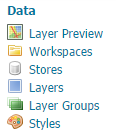
\includegraphics[width=0.25\textwidth]{Figures/Data.png}
	  \vspace{-10pt}
	\caption{\label{fig:data}Data section of navigator}
	  \vspace{-10pt}
\end{wrapfigure}
This section gives a step by step guide of how to create a visual
geospacial representation using the pre-aggregated index of the example
dataset. This will be done using GeoServer, specifically the GeoServer web
administration interface. This section offers are concrete version of the
deployment discussed in \Fref{sec:deployment}.

\Fref{fig:data} shows the \lstinline|Data| section of the navigator which
can be found on the left hand side of the web administration interface. The
links in this section will be used to navigate between different pages
needed to configure the whole setup.

\subsubsection{Add Source}

\begin{figure}[t]
	\centering
	\subfigure[Add new store \label{fig:newstore}]{
		\raisebox{8mm}{
		
\includegraphics[scale=0.6]{Figures/AddNewStores.png} }}
	\subfigure[Select data source type \label{fig:storetype}]{
		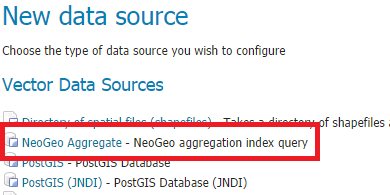
\includegraphics[scale=0.6]{Figures/StoreType.png} }
	\caption{Adding new \lstinline|Store| to GeoServer}
\end{figure}

\begin{figure}[p]
	\centering
	\subfigure[\label{fig:createstore}\lstinline|New Vector Data Source|]{
		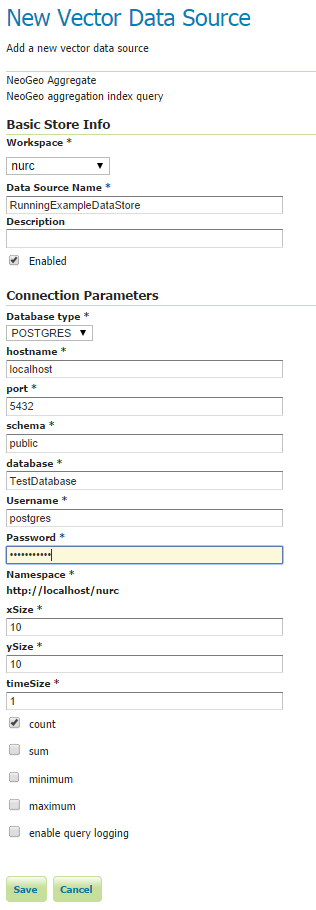
\includegraphics[width=.4\textwidth]{Figures/CreateStore.png}}
	\subfigure[\label{fig:editlayerdata}\lstinline|Edit Layer| page]{
		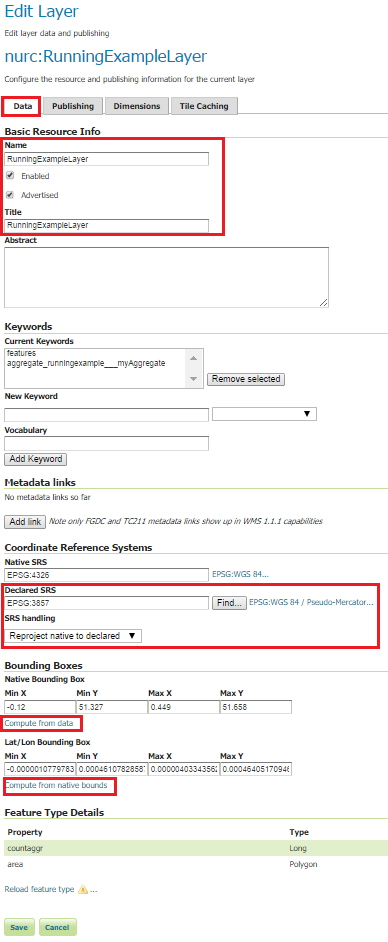
\includegraphics[width=.5\textwidth]{Figures/EditLayer_Data.png}}
	\caption{Configuring a store and layers\label{fig:storeandlayers}}
\end{figure}

A data source is added in the following way:
\begin{enumerate}
	\item Click on the \lstinline|Stores| link in the \lstinline|Data|
		section shown in \Fref{fig:data}.
	\item The \lstinline|Stores| will open, the top of the page looks like
		\Fref{fig:newstore}; click on the \lstinline|Add new Store| link.
	\item A selection of different \lstinline|Vector Data Sources| is now
		available. Select \lstinline|NeoGeo Aggregate| as shown in
		\Fref{fig:storetype}. 
\end{enumerate}

\begin{enumerate}[resume]
	\item After selecting \lstinline|NeoGeo Aggregate| as
		\lstinline|Vector Data Source| a page like \Fref{fig:createstore}
		will open. Fill in all the fields as shown. Some values may differ
		depending on how the database is setup. More exact information can
		be found in \Fref{sec:addingsource}.
	\item Once everything is filled out click the \lstinline|Save| button.
		This leads to page where \lstinline|Layers| can be published.
		However before that is done, first the \lstinline|Style| should
		be imported.
\end{enumerate}

\subsubsection{Import Style}

Importing a style is done as follows:
\begin{enumerate}[resume]
	\item Click on the \lstinline|Styles| link in the \lstinline|Data|
		section shown in \Fref{fig:data}.
	\item Click on the \lstinline|Add a new style| button which will go to a
		page similar to \Fref{fig:styleimport} although empty.
	\item Import the \lstinline|RunningExampleSLD.xml| file by using the
		\lstinline|Choose File| button. The \lstinline|Upload...| link
		is highlighted in red in \Fref{fig:styleimport}.
	\item Once the style has been uploaded, the \lstinline|New style| page
		should look like \Fref{fig:styleimport}.
	\item Press the \lstinline|Save| button.
\end{enumerate}
The style used in this example has been imported in GeoServer and now the
layer is ready to published.

\begin{figure}[t]
	\centering
	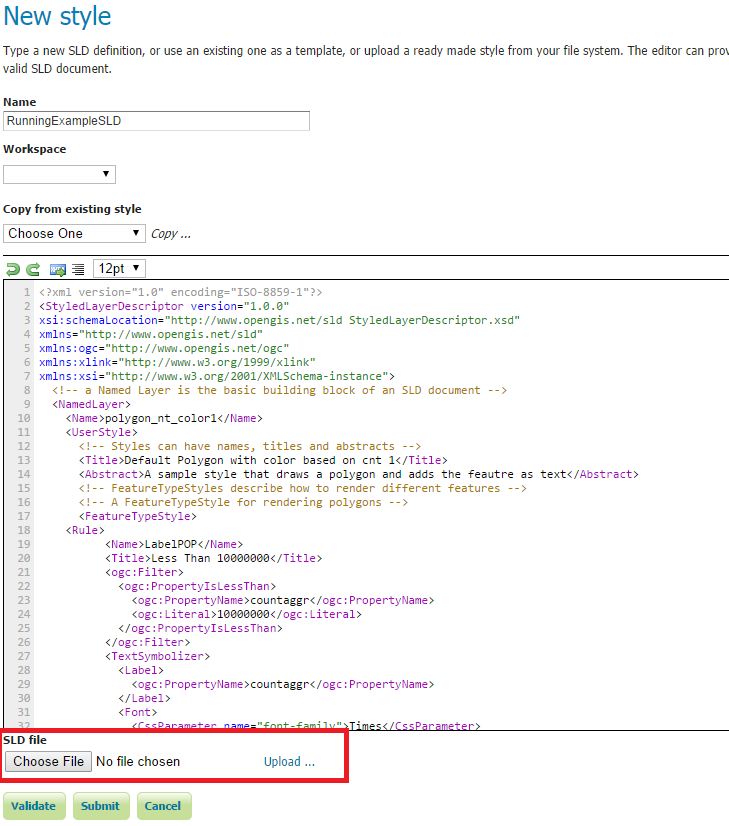
\includegraphics[scale=0.5]{Figures/NewStyleImport.png}
	\caption{\label{fig:styleimport}Importing SLD style from file}
\end{figure}

\subsubsection{Create Layer}

\begin{figure}[t]
\centering
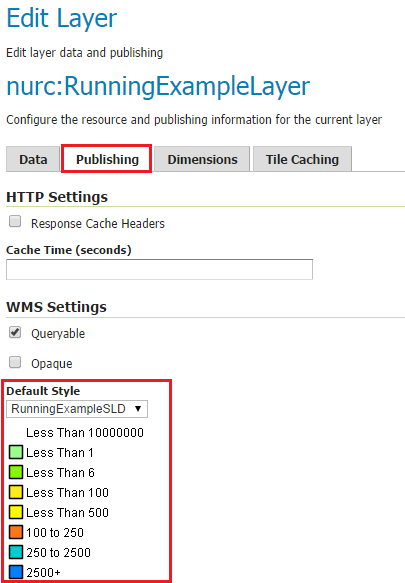
\includegraphics[width=0.5\textwidth]{Figures/EditLayer_Publishing.png}
\caption{Adding a \lstinline|Style| to the \lstinline|Layer|
\label{fig:layerpublish}}
\end{figure}

\begin{figure}[t]
	\centering
	\includegraphics[width=\textwidth]{Figures/Publishlayer.png}
	\caption{Publishing a \lstinline|Layer|\label{fig:publishlayer}}
\end{figure}

Creating a new layer is done as follows:

\begin{enumerate}[resume]
	\item Click on the \lstinline|Layers| link in the \lstinline|Data|
		section shown in \Fref{fig:data}.
	\item This opens the \lstinline|Layers| page, here click on the
		\lstinline|Add a new resource| button. This open a page similar to
		\Fref{fig:publishlayer}.
	\item Select the \lstinline|Publish| action for the example layer.
	\item A page like \Fref{fig:editlayerdata} will open. Set highlighted
		fields to match \Fref{fig:editlayerdata}. More exact information
		about these fields can be found in \Fref{sec:addinglayers}.
	\item After the fields in the \lstinline|Data| are filled in, go to
		the \lstinline|Publishing| tab, see \Fref{fig:layerpublish}.
	\item Set the default style to \lstinline|RunningExampleSLD| like
		in \Fref{fig:layerpublish}.
	\item Press the \lstinline|Save| button.
\end{enumerate}

A layer for the example dataset has now been created and is ready to be
viewed.

\subsubsection{View Layer}

\begin{figure}[t]
\centering
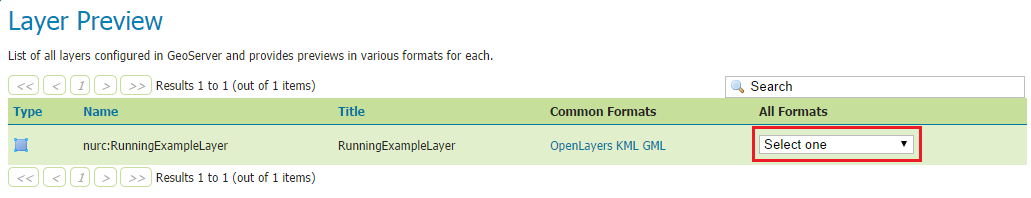
\includegraphics[width=\textwidth]{Figures/LayerPreview.png}
\caption{Previewing a \lstinline|Layer|\label{fig:preview}}
\end{figure}

The final GeoServer step is to preview the layer. The preview only shows
the highest granularity of the aggregation index. Getting a preview of a
layer is done as follows:
\begin{enumerate}[resume]
	\item Click on the \lstinline|Layer Preview| link in the
		\lstinline|Data| section shown in \Fref{fig:data}.
	\item The \lstinline|Layer Preview| page opens which displays all
		viewable layers like in \Fref{fig:preview}.
	\item A preview format need to be selected from the drop-down menu
		highlighted in \Fref{fig:preview}.
	\item Select a \lstinline|WMS| preview format such as \lstinline|PNG|.
	\item A new web page will load (this might a few seconds depending on
		whether or not the server side extension is enabled).
	\item The final result will look like \Fref{fig:result}.
\end{enumerate}

The layer showing the example dataset is now complete. The values of
each square in the layer is calculated using the pre-aggregate index of the
dataset. See \ref{sec:clientsidedev} to learn how the layer can be used in
combination with other tools such as
OpenLayers\footnote{\url{http://openlayers.org/}} to create a dynamic map
which updates data on the fly.

\begin{figure}[t]
\centering
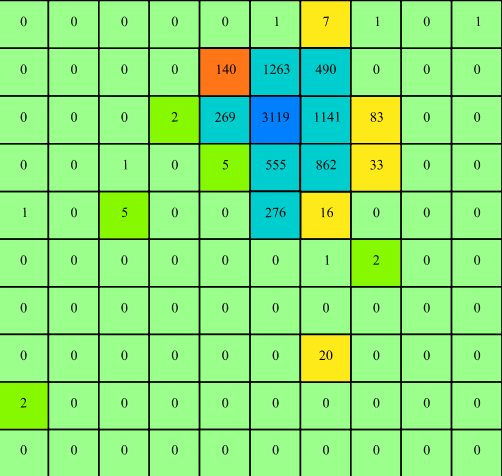
\includegraphics[width=0.45\textwidth]{Figures/FinalResult.png}
\caption{Preview of whole dataset \label{fig:result}}
\end{figure}



\end{document}
